\documentclass[12pt]{article}
\usepackage{graphicx}
\usepackage[letterpaper,margin=1in]{geometry}
\usepackage[utf8]{inputenc}
\usepackage{hyperref}
\begin{document}
\title{Letter from M Carley}
\author{Alan R. Rogers}
\date{14 February 2021}
\maketitle

This document contains a letter that has been folded up inside a bible
that once belonged to Robert Walker Carley, who was born May 22, 1834,
in Ireland and died Aug.\ 5, 1872, in Seguin, Texas, at the age of
38. At the time of his death, Carley was Rector of St.\ Andrews
Episcopal Church. A summary of Carley's life can be found
\href{https://www.newspapers.com/clip/21483199/robert-walker-carley-bio-from-seguin}{here}.

Although the letter is addressed only to ``My Dear Child,'' I suspect
it was sent to Margaret Alice Carley, the daughter of Robert
Carley. It is signed, ``your loving and affectionate mother,''
followed by what looks to me like ``M Carley.'' Alice's biological
mother had died when she was about two years old, so this letter must
be from her step-mother, Fannie Lamont Carley, whom Robert had married
on March 14, 1867. Perhaps the ``M'' stands for ``Mother,'' or maybe
it isn't really an ``M.''

This letter seems to be on the same stationary as
\href{./RobtCarley.pdf}{the one} from Robert Carley, so I suspect it
was written at about the same time, in 1868.

Here is my best effort at a transcription:
\begin{quotation}
  \noindent My Dear Child,

  I am really glad to hear your Father found you in such good health
  and spirits. I trust you take good care of your health its well
  worth your care, I am so sorry the weather is to rough it
  [undecipherable] prevents yourself and your Father enjoying the
  beauties of your neighborhood he was busy climbing some of the
  mountains before he left us but when it has happened so you can make
  [missing line] [how?] strait collars on your shirts send me the
  soiled ones by your father and if you [indecipherable] of repair
  send them [undecipherable]. Tell the Laundress that these collars
  require to be very stiff and also well pressed on the inside to
  prevent their being uncomfortable. I trust your father and yourself
  will continue in good health and that he will be home safely on
  Friday, your winter stockings must want mending very badly send them
  to me I will send them back in a few days the little ones all join
  me to you and their father. Your loving and affectionate mother,
  M. Carley. 
\end{quotation}
I would welcome corrections or additions to this transcription


\bigskip

\mbox{}\hfill Alan R. Rogers\\
\mbox{}\hfill sregorra@gmail.com\\

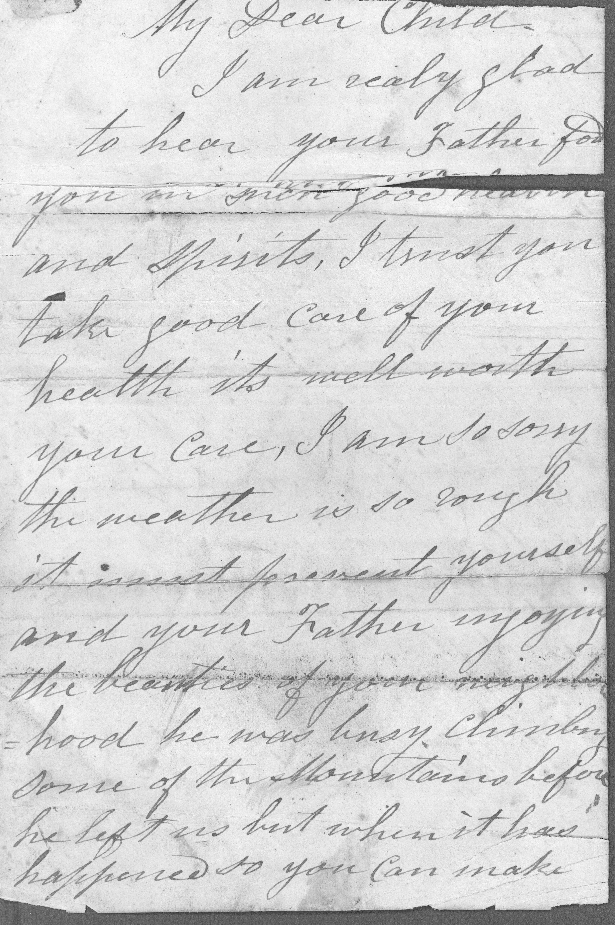
\includegraphics[width=\textwidth]{MCarley1.pdf}
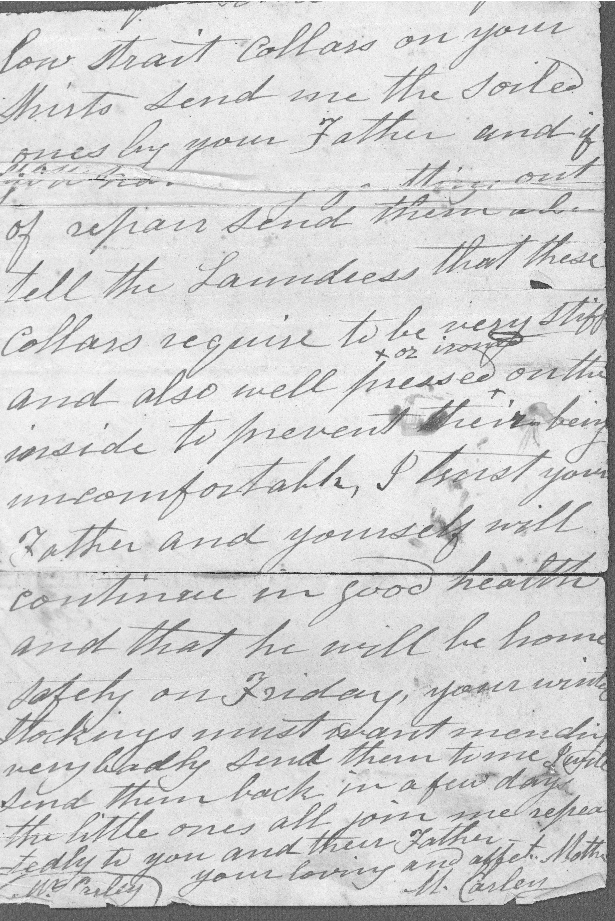
\includegraphics[width=\textwidth]{MCarley2.pdf}
\end{document}
